\documentclass[10pt]{article}
\usepackage[margin=1in]{geometry}
\usepackage{graphicx,booktabs,amsmath,hyperref,microtype}
\usepackage[numbers]{natbib}
\title{The Recipe, Not the Data: An Audited Ledger of Physics\\Identifiability in a Structured World Model}
\author{Cesar Augusto\\\small\texttt{github.com/cesaremcasa/Atlas.WM}}
\date{Draft v0.1 --- July 2026}

\begin{document}
\maketitle

\begin{abstract}
We present an end-to-end audited study of physical-parameter identifiability in a
small structured world model, across a toy 2D environment and a MuJoCo
contact-physics environment. Our starting point is a retraction: the project's
previous conclusion --- that a friction parameter was ``not identifiable'' under
random exploration --- was wrong, caused by an uncommitted evaluation oracle whose
MSE objective was destroyed by heavy-tailed collision outliers, compounded by a
simulator bug that silently voided the physics signal. Re-verifying every claim
produced a three-step thesis, each step measured under episode-held-out
evaluation: (1)~\emph{the information exists} --- a robust closed-form estimator
recovers friction at $R^2{=}0.87$ from the same noisy data where a GRU belief
encoder scores $-0.49$; (2)~\emph{features unlock learning} --- handing the
estimator's sufficient statistics to the same GRU flips all three parameters
positive (gravity $+0.43$); (3)~\emph{collection amplifies} --- an
information-seeking policy improves belief quality $+39\%$ over random data with
the model held fixed. The thesis transfers to MuJoCo contact physics (friction
$+0.28$, mass $+0.11$ from a zero baseline), where analysis also yields a
structural identifiability result (only the $\mu g$ product enters box dynamics)
and a cautionary finding: deterministic information-seeking policies require
\emph{anti-fragility to unobservables}. All claims map to committed scripts,
seeded runs, and regression tests.
\end{abstract}

\section{Introduction}
Negative identifiability results in world-model research are commonly attributed
to the \emph{data regime}. We document a case where that conclusion was published
in a project's model card and was wrong three ways at once: the supporting oracle
was never committed (unreproducible), its objective was statistically fragile
(MSE under heavy-tailed outliers), and the environment itself had a bug that
removed the signal being measured. Rather than merely fixing the record, we use
the retraction as a method: every subsequent claim is (i)~reproduced by a
committed script, (ii)~evaluated with episode-grouped splits (row-level splits
leak episode labels through overlapping windows --- we measure the leak at
$R^2{\approx}0.3$ on pure noise), and (iii)~guarded by a regression test.

\section{Setup}
\textbf{Environments.} (a)~\emph{CruelGridworld}: three bodies on a bounded plane,
nonlinear inter-object attraction ($G/d^2$, active $1{<}d{<}10$), per-episode
gravity/friction randomization, process noise $\sigma{=}0.05$, 8 discrete force
actions, 6-D position-only observations. (b)~\emph{MujocoPointMass}: an actuated
ball and two passive boxes on a bounded MuJoCo plane; episode latents are sliding
friction, box masses and gravity; same discrete action interface plus a no-op.
\textbf{Belief model.} A GRU over $K$-step same-episode windows (RMA/VariBAD
lineage \citep{kumar2021rma,zintgraf2020varibad}) with a heteroscedastic Gaussian
head and an optional half-window InfoNCE episode-contrastive term.
\textbf{Protocol.} Episode-grouped splits throughout; supervised held-out $R^2$
per parameter; fully seeded training with a bit-identical canary test.

\section{A retraction as a methodology lesson}
A committed median-of-ratios estimator on position-only observations --- per-step
decay ratios $\langle v', v{+}\alpha u\rangle/\lVert v{+}\alpha u\rVert^2$, gated
by excitation, boundary-bounce and interaction filters, aggregated by the median
--- recovers friction at $R^2{=}0.865$ (MAE $0.006$) on the same noisy
random-policy data previously declared uninformative. The original oracle failed
because collisions create heavy-tailed ratio outliers: a least-squares fit of the
identical quantity scores $R^2{=}-35$. Separately, a containment bug let passive
boxes exit the arena, silently removing the interaction signal. \emph{Negative
identifiability claims inherit every fragility of their oracle and their
simulator.}

\section{The three-step thesis}
\textbf{Step 1 --- the information exists.} The closed-form estimator sets the
reference (friction $0.865$); the GRU on raw windows scores $-0.49$ on the same
data while its training loss decreases --- episode memorization, not learning.
\textbf{Step 2 --- features unlock learning.} Handing the GRU the estimator's
sufficient statistics (gated decay ratio and its running median, excitation,
distances, attractor-projected box accelerations, $1/d^2$ regressors, aligned
actions) flips all three parameters positive (Fig.~\ref{fig:thesis}). Two
measured failure modes: a single misaligned action index nullifies every ratio;
and an \emph{evidence-length bound} --- the target's std ($0.025$) lies below the
optimal estimator's window-level error at 18 steps ($0.043$), so no learner can
score positive there. \textbf{Step 3 --- collection amplifies.} An
information-seeking policy raises belief quality $+39\%$ with the model fixed
(gravity $0.67$). Its first version dashed along a fixed line and repeatedly
struck an unobservable obstacle, poisoning the episode median (Fig.~\ref{fig:af});
a golden-angle rosette restores robustness --- \emph{anti-fragility to
unobservables}.

\begin{figure}[t]\centering
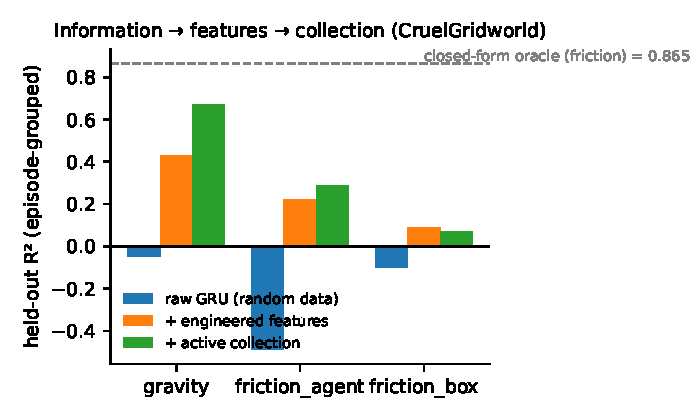
\includegraphics[width=.62\linewidth]{figures/fig1_thesis.pdf}
\caption{The three-step thesis on CruelGridworld: same GRU, same evaluation;
only features and data collection change.}
\label{fig:thesis}
\end{figure}

\begin{figure}[t]\centering
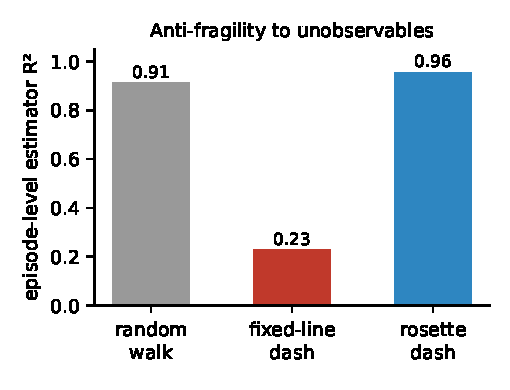
\includegraphics[width=.4\linewidth]{figures/fig4_antifragility.pdf}\hfill
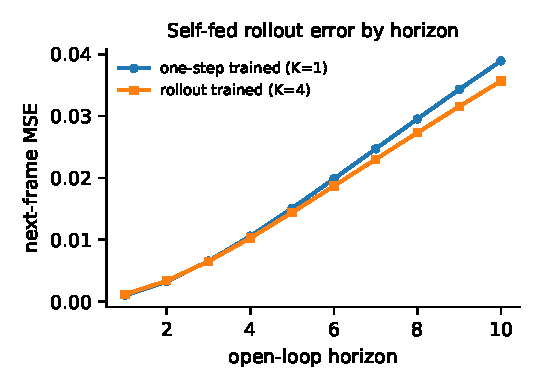
\includegraphics[width=.42\linewidth]{figures/fig3_horizon.pdf}
\caption{Left: deterministic information-seeking must be robust to
unobservables. Right: rollout-trained world models trade one-step accuracy for
slower open-loop degradation.}
\label{fig:af}
\end{figure}

\section{Transfer to MuJoCo contact physics}
Random policy $+$ generic statistics: $R^2{\approx}0$ on all parameters. Analysis
explains why: the actuated agent rides slide joints (normal force ${\approx}0$;
it slides nearly frictionless), so only the boxes feel friction; Coulomb friction
decelerates \emph{linearly} (ratio features are the wrong model class); and
gravity enters box dynamics only through $\mu g$ --- \emph{structurally
unidentifiable alone}, an exclusion made with a measurement rather than by
assertion. A COAST/PUSH policy (no-ops manufacture free sliding; box-directed
pushes manufacture contacts) plus aligned-impulse features (head-on contacts
only; glancing hits confound geometry with mass at $-0.27$) yields learned
beliefs of friction $+0.28$ and mass $+0.11$ at 1{,}048 episodes
(Fig.~\ref{fig:mj}).

\begin{figure}[t]\centering
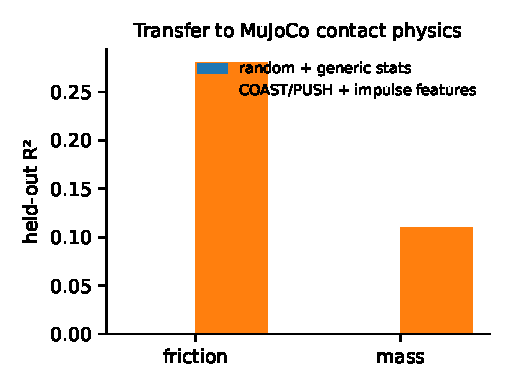
\includegraphics[width=.42\linewidth]{figures/fig2_mujoco.pdf}
\caption{The thesis transfers to real contact physics.}
\label{fig:mj}
\end{figure}

\section{Related work}
Belief-style system identification: RMA \citep{kumar2021rma}, VariBAD
\citep{zintgraf2020varibad}. Active system identification: ASID
\citep{memmel2024asid} --- our policies replace the Fisher objective with
measured information-rate proxies. Self-predictive stability:
\citet{ni2024bridging}; our world model uses VICReg-style regularization
\citep{bardes2022vicreg} plus prediction grounding. Our contribution is an
audited, fully reproducible account connecting these pieces, with retraction,
failure ledger, and structural identifiability analysis.

\section{Limitations}
Two synthetic environments; no visual observations; policies are designed, not
learned; the world model sits $2.3\times$ above its linear information ceiling on
MuJoCo; mass identification remains weak ($+0.11$).

\bibliographystyle{plainnat}
\begin{thebibliography}{9}
\bibitem[Kumar et al.(2021)]{kumar2021rma} A. Kumar, Z. Fu, D. Pathak, J. Malik.
RMA: Rapid Motor Adaptation for Legged Robots. \emph{RSS}, 2021.
\bibitem[Zintgraf et al.(2020)]{zintgraf2020varibad} L. Zintgraf et al. VariBAD:
A Very Good Method for Bayes-Adaptive Deep RL. \emph{ICLR}, 2020.
\bibitem[Memmel et al.(2024)]{memmel2024asid} M. Memmel et al. ASID: Active
Exploration for System Identification. \emph{ICLR}, 2024.
\bibitem[Ni et al.(2024)]{ni2024bridging} T. Ni et al. Bridging State and History
Representations: Understanding Self-Predictive RL. \emph{ICLR}, 2024.
\bibitem[Bardes et al.(2022)]{bardes2022vicreg} A. Bardes, J. Ponce, Y. LeCun.
VICReg: Variance-Invariance-Covariance Regularization. \emph{ICLR}, 2022.
\end{thebibliography}
\end{document}
